\chapter{Real Time Radio Astronomy Algorithms}
\label{chap:Real Time Radio Astronomy Algorithms}
%Summary: Give an description of radio astronomy instrumentation \\
%Describe science goals and mathematical function \\
%Goal: Give background for the application. Show that most instruments use a small number of high level functions\\
%State: Can be written now \\
%Use info from casper papers and radio 101 \\
%References already compiled \\

%Radio Astronomy Problems
%Are we alone?
%When were the first stars and galaxies formed?
%Galactic structure and formation (mapping the galaxy)
%Nature of gravitational wave background (pulsar timing)
%Transient universe
%Black hole imaging
%Searching for extrasolar planets



Radio astronomy simply refers to the type of science that can be done by observing astronomical objects at radio wavelengths, rather than a specific scientific goal. 
There is a huge variety of different experiments, such as studying the formation and structure of galaxies stars and black holes and searching for gravity waves, traces of the first stars \cite{Parsons:2009vg}, or aliens \cite{1995ASPC...74..293W}.
But, despite this variety, the small number of algorithms detailed in this chapter serve as the first step in processing the data for many such projects.



Radio telescopes produce very high amounts of data. %(TODO: add estimates, how much data?). 
The reason for this high influx of data is twofold. 
First, to enable new science, new radio antennas observe increasingly higher bandwidths. 
%TODO edit this
%TODO: and to surveil a large part of the sky
Second, to sate the need for larger collecting area, rather than designing a single large dish, many new telescopes are being designed as antenna arrays, where the data from multiple antennas is combined to act as a single large dish.
While it may be cheaper and easier to get a larger collecting area using small dishes rather than a single large dish, this adds additional complexity processing the data coming off the telescope.
Rather than processing a single stream of data, now the instrument must process and combine multiple streams to make the array seem like a single large dish.
As the size of the arrays and bandwidths for single dishes simultaneously increase, the data produced cannot be feasibly recorded in real-time. 
To cope with the progress in science and antenna technology, there is a constant need for new systems to process, rather than record, this data in real time.
Each of these instruments begin processing the data immediately after it is digitized, and need to reduce the data without losing scientific information.
Once the data is partially processed, and reduced to a manageable bandwidth, it can be stored and processed further offline.
%, where there is no longer a need for low-latency, high-bandwidth hardware.


%\section{Real Time Algorithms}
%TODO add complexity analysis
There are a small number of real time algorithms commonly used to reduce the data. 
In this work, we specifically focus on spectroscopy, pulsar processing, beamforming and correlation. 
Spectroscopy and pulsar processing are both spectral methods of analyzing data from a single beam.
They both can be used on antenna arrays but would either need to treat the array as separate dishes rather than one large dish, or the data from the dishes would need to be combined into a single beam, which can be done using the third algorithm on the list, beamforming. 
The last two techniques, beamforming and correlation, are both ways of combining data from multiple antennas. 
Beamforming combines the data into a single beam by delaying and summing the data from each antenna.
Correlation doesn't aim to form a single beam, but instead is the first step towards getting an image of the sky. 



%TODO: Discuss full stokes/dual pol spectrometer
\section{Spectroscopy}
\label{Real Time Radio Astronomy Algorithms:Spectroscopy}
A spectrometer is simply an instrument that produces an integrated, or averaged, frequency domain spectrum from a time domain signal. 
A real time spectrometer works by constantly computing a spectrum over short windows of data (channelization), then each channel is summed for a predetermined amount of time to compute the average power in that channel (accumulation). 
%Figure x shows a block diagram for a simple spectrometer design. 
%(TODO: add spectrometer block diagram)
After digitization, there is the channelization step, where the signal is processed by a digital filter bank, and then the channels are accumulated. 

\subsection{High resolution spectroscopy}
Increasing resolution often requires an increase in complexity in the spectrometer design. 
Once the number of required channels is sufficiently high, it becomes infeasible to compute the spectrum using a single filter bank. 
To cope with this, the channelization is done in two steps. % as shown in figure. 
In the first step, the signal is divided into coarse channels using a filter bank. 
At this point the channels are much wider than intended and can't be accumulated yet. 
After coarse channelization, the spectrometer treats the data from a single channel as time domain data and passes it through a filter bank again. 
This step breaks up the wide channel into a number of smaller channels. 
At this point the data can be accumulated, since it has the desired resolution.

\subsection{Applications}

This high resolution spectroscopy technique is used in the SERENDIP V.v (Search for Extraterrestrial Radio Emissions from Nearby Developed Intelligent Populations) project. 
This project is part of the SETI (Search for Extraterrestrial Intelligence) effort to detect extraterrestrial intelligence. 
The SERENDIP V.v project is a commensal survey at the Arecibo observatory, meaning anytime the ALFA receiver is used for any observation, the SERENDIP spectrometer will also process and record data. %TODO: add time estimate 

The project is focused on detecting strong narrow band radio signals, requiring a high resolution spectrometer installed at the observing telescope to analyze the data. 
The spectrometer should resolve channels of less than 2 Hz, so that natural astronomical signals that typically have a wider bandwidth can easily be distinguished from narrower, possibly extraterrestrial, signals. 
The SERENDIP V.v spectrometer meets this by providing 128 million channels across 200 MHz of bandwidth, for an resolution of 1.5 Hz per channel. 
Since it would be infeasible to channelize a 200 MHz signal into 128 million channels using a single filter bank, the SERENDIP V.v spectrometer uses the high resolution architecture described in Chapter \ref{chap:Related Work}. %TODO: add reference to diagram

%TODO add scaling info





\section{Pulsar Processing}
\label{Real Time Radio Astronomy Algorithms:Pulsar Processing}
A pulsar processor is an instrument designed specifically to observe transient events, such as pulsars. 
A pulsar is a rotating neutron star that emits an electromagnetic beam. 
When the beam sweeps past Earth, due to the rotation of the star, it is observed as a pulse of wideband noise. 
As the pulse travels through the interstellar medium (the matter filling interstellar space), the signal gets dispersed, meaning the low frequencies arrive before high frequencies, despite the fact that they were emitted at the same time. 

%TODO: event horizon telescope
\begin{wrapfigure}{L}{0.50\textwidth}
  \centering
    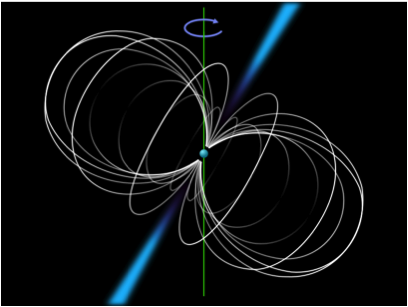
\includegraphics[width=0.49\textwidth]{Images/C2/pulsar.png}
  \caption{A Conceptual Pulsar Diagram}
  \label{fig: C2/pulsar.png}
\end{wrapfigure}

A spectrometer, as described in Section \ref{Real Time Radio Astronomy Algorithms:Spectroscopy}, that accumulates the spectrum would smear the pulse, so there will need to be a few adjustments to the spectroscopy algorithm to make it suitable for processing transient events. 
In the case of pulsars, the algorithm starts with a high-resolution spectrometer without an accumulator. 
Instead, the algorithm becomes specialized to detect this type of quickly occurring event.

The high resolution data is then sent to a process called dedispersion, which undoes the dispersion caused by the ISM, realigning the pulse.
%TODO: describe dm, pulsar searching
There are 2 techniques to do this.
First, the pulse can be dedispersed by shifting the frequency channels by different amounts to compensate for the different delays, in a process called \emph{incoherent dedispersion}. %TODO: add figure,
This process can't be used to reconstruct the original pulse, but due to its relatively low compute cost, is a useful algorithm to search for new pulsars.
The second technique, \emph{coherent dedispersion}, models the effect of the ISM as a convolving filter. 
To remove this effect, the signal is deconvolved with the model.
This is more compute intensive than incoherent dedispersion, but can recover the original pulse.

After dedispersion, there is a still a lot of data and the pulse has very low SNR. 
The next step in processing is \emph{folding}, or adding together many pulses, reducing the amount of data and improving the SNR.
At this point, the data has been significantly reduced and can be recorded. 

%TODO add scaling into

%TODO: Graphic to describe this process. Block diagram + images

%Detect dispersed pulses
%
%TODO: add science info
\subsection{Applications}
Some pulsars serve as very accurate astronomical time keepers.
There are millisecond pulsars with extremely stable periods, allowing any perturbations in the observed pulse period to be attributed to some external effect.
This makes pulsars extremely useful for conducting relativity experiments. 
One such example is the North American Nanohertz Observatory for Gravitational Waves, or NANOGrav, Project, %TODO: add citation The international pulsar timing array project: using
which uses pulsars in an attempt to make the first detection of gravitational waves \cite{2009astro2010S..64D}. 
The project will try to detect gravitational waves by observing an array of pulsars, measuring the effect of the waves passing between Earth and the pulsars as changes in observed pulse arrival times.

%TODO: diamond planet
%\begin{wrapfigure}{L}{0.50\textwidth}
%  \centering
%    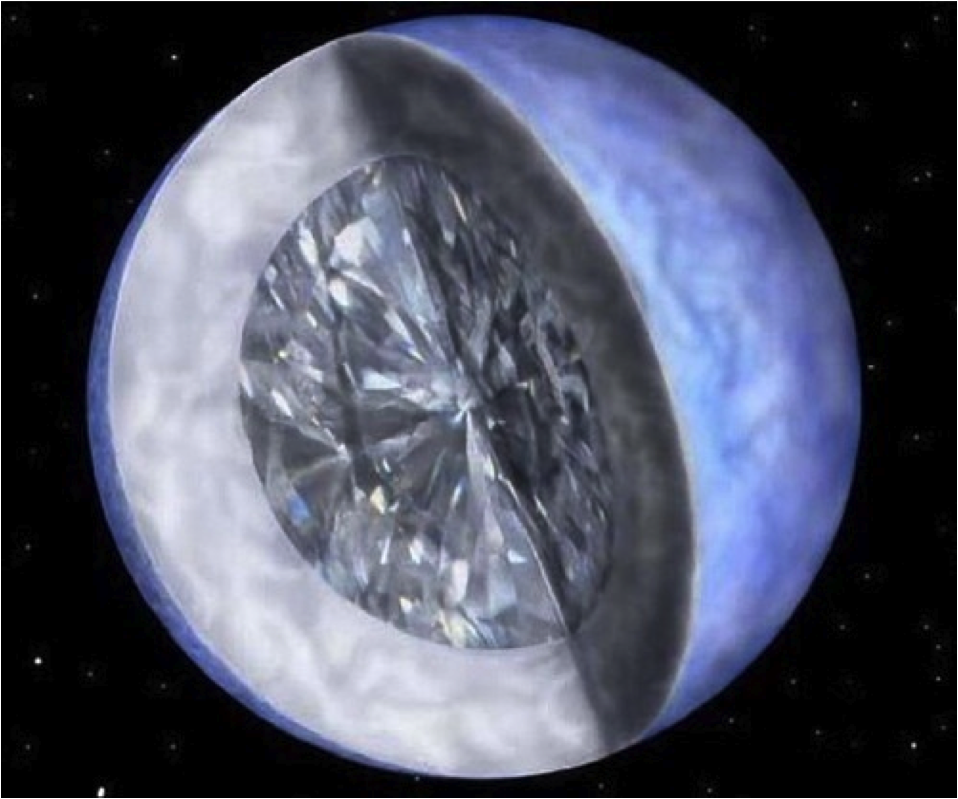
\includegraphics[width=0.49\textwidth]{Images/C2/diamond_planet.png}
%  \caption{TODO}
%  \label{fig: C2/diamond_planet.png}
%\end{wrapfigure}

%Beyond astronomy, pulsars could also serve as 

\section{Beamforming}
\label{Real Time Radio Astronomy Algorithms:Beamforming}
Beamforming is a technique for combining data from an array of antennas.
The beamformer combines the data from multiple antennas into a single beam pointed at a single point in the sky.
This is achieved by delaying the signal from each antenna by a different amount and then summing the delayed signals. 
The signal from the intended source will not arrive at all the antennas at the same time. 
The delay compensates for the disparity between the arrival times, and once the signals are summed it creates constructive interference in the direction of the source, and destructive interference in other directions. 
These delays can be changed to point the beam at a different source or to track a single source moving across the sky.


\subsection{BF Beamforming}
%TODO: revisit this sentence
Since the digitized signal from a radio telescopes receiver is discrete, and the amount of delay might not be an integer multiple of the sample period $s$, the delay $d$ is applied to the signal, $f[n]$, in 2 steps. 
The delay in clock cycles is represented as $d/s$ and broken up into it's integer and fractional parts. 
First, the integer part is applied as a coarse delay, $n_f = \lfloor d/s \rfloor$. 
This can simply be implemented by buffering the signal.
Applying the  fractional delay $d \bmod s$ is more complex. 
Since there is no observed data at that time, the signal fractional samples are calculated by convolving the signal with an interpolation filter $b$.
Applying these 2 steps, results in a new delayed signal $f[n] = f[n-n_f]\ast b_{fi}$

In practice, it is common to calculate the spectrum of the beamformed signal. 
%TODO: explain why spectrum is desirable
A typical 2 element beamformer, with discrete input signals $f[n]$ and $g[n]$ is trying to calculate the spectrum of beam $i$, $H_i$, using coarse delays $n_{fi}$  $n_{gi}$ and delay filters $b_{fi}$ and $b_{gi}$, as follows: 
\[H_i(x) = FT(f[n-n_{fi}]\ast b_{fi} + g[n-n_{gi}]\ast b_{gi})\]
We describe this as BF beamforming because the delay operation (B), happens before the FT operation (F).

%TODO add info on scaling here

\subsection{FB Beamforming}
In the case where many beams are required, each beam needs a different FIR filter for every antenna, and a separate Fourier transform. 
This is called FB beamforming because the fourier transform operations (F) occur before the delay (B). 
Using linearity of the Fourier transform and the convolution theorem, the computation can be rearranged as follows:

%TODO fix this
%\begin{align*}
%H_i(x) &= FFT(f[t-t_{fi}]) \cdot FFT(b_{fi}) + FFT(g[t-t_{gi}]) \cdot FFT(b_{gi}) \\
%&= F[x] \cdot B'_{fi} + G[x] \cdot B'_{gi} \\
%\end{align*}
\[H_i[x] = F[x] \cdot B'_{fi} + G[x] \cdot B'_{gi}\]

Where $F[x]$ and $G[x]$ are the fourier transforms of the signals $f$ and $g$.
The signal delay becomes a phase shift in frequency domain that is represented by $B'_{fi}$ and $B'_{gi}$. 
In this case, there is a FT for each antenna, rather than one FT per beam. 
When forming multiple beams, there is no need to recalculate the Fourier transform of the signals. 
%$A$ signals, $n$ frequency channels, $B$ beams and a $$
So, as the number of beams increases, it can be advantageous to use this algorithm rather than the BF algorithm described in the previous section. 

%\subsection{Applications}
%Forming beams improves the signal to noise ratio of the \cite{2012Sci...338..355D}
%TODO add info on scaling here

%TODO: Add 2 element beamformer
%%Add together multiple (delayed) signals to improve SNR

%TODO: event horizon telescope
%\begin{wrapfigure}{L}{0.50\textwidth}
%  \centering
%    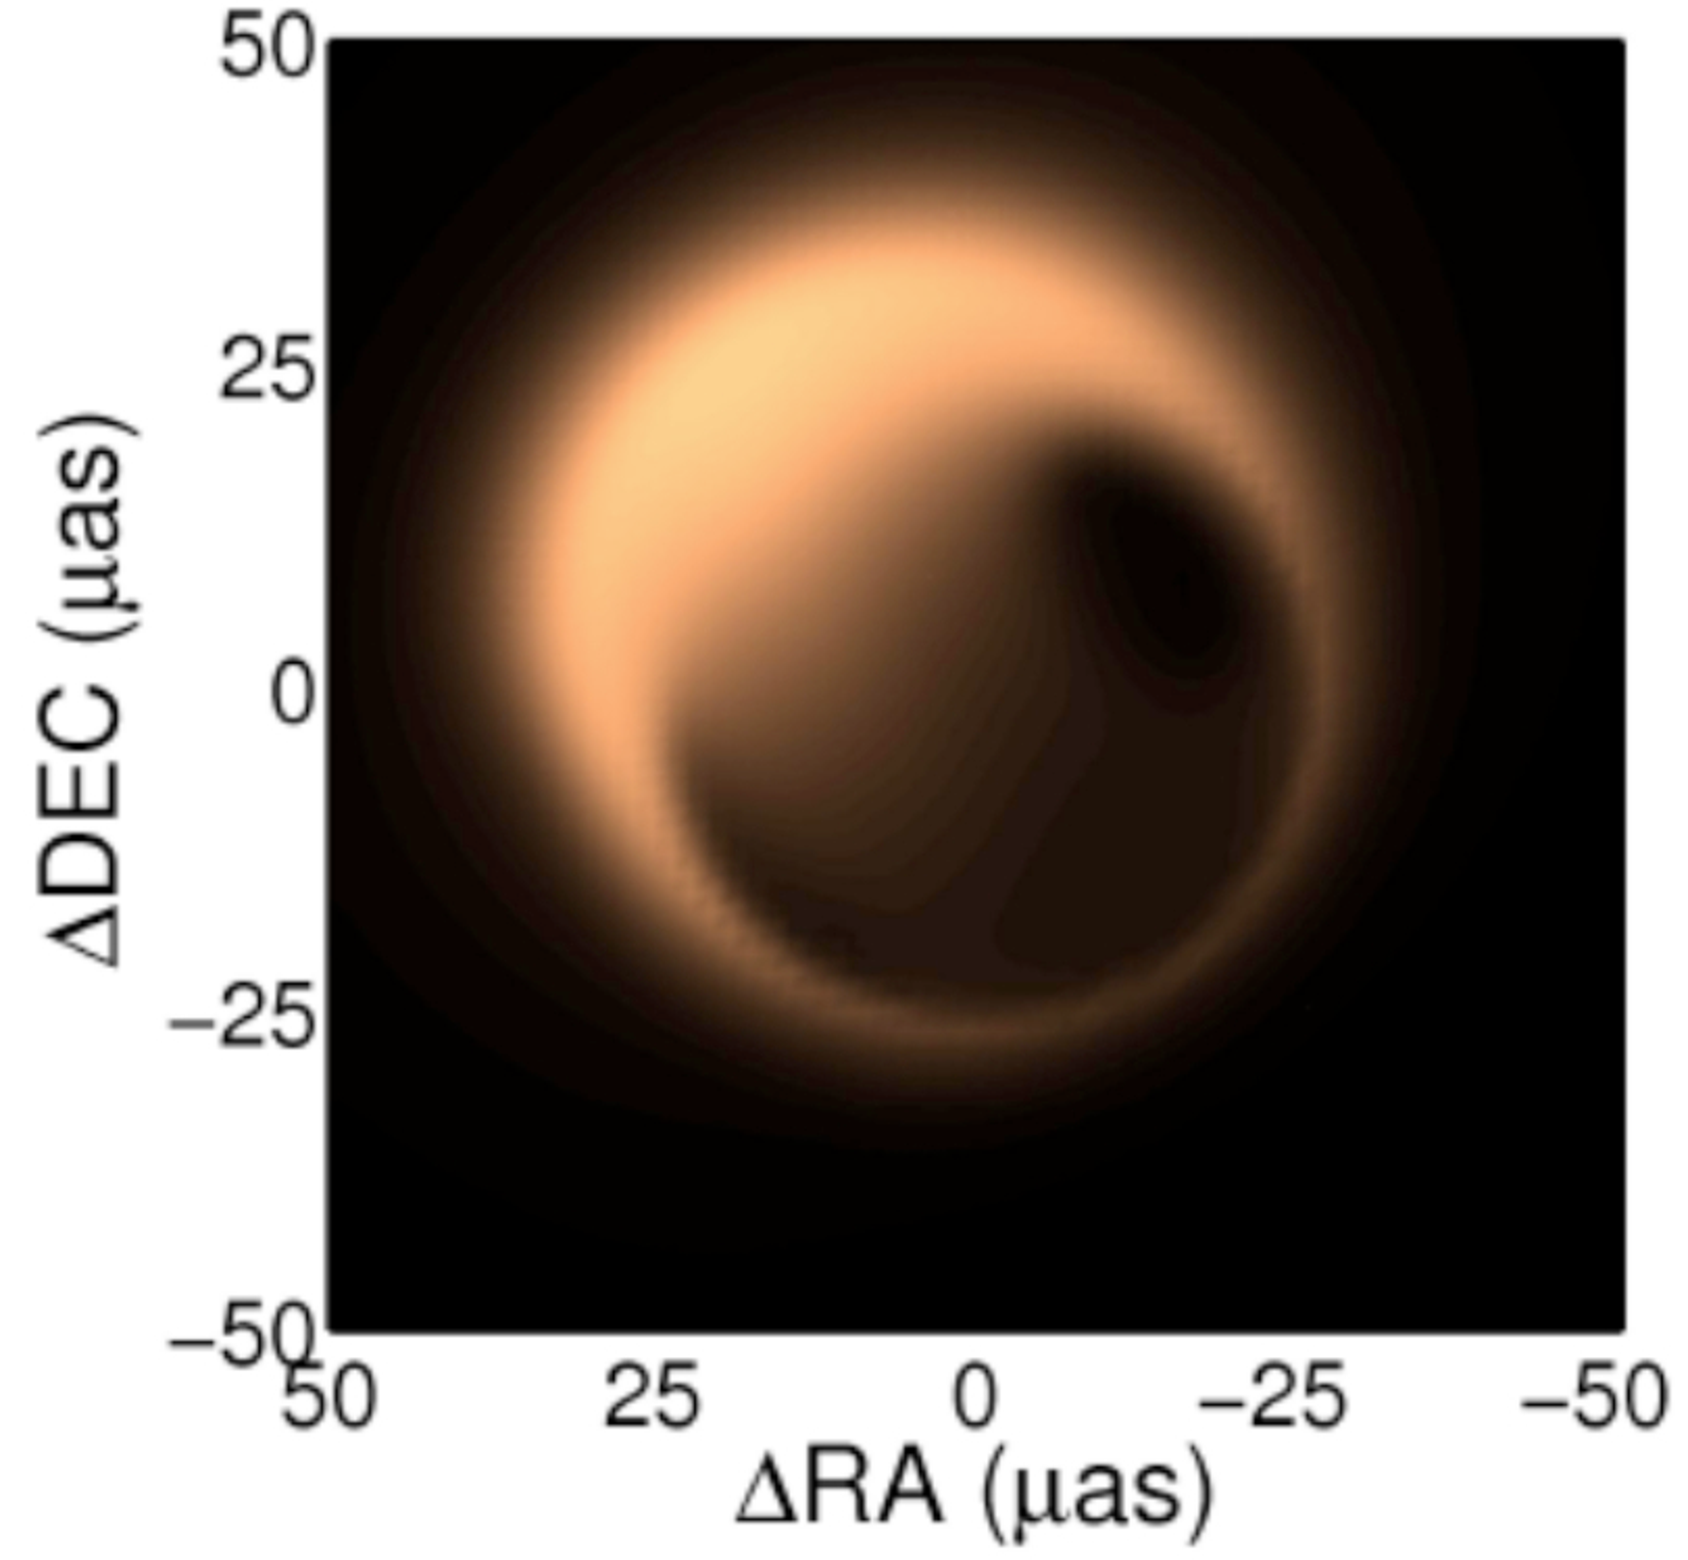
\includegraphics[width=0.49\textwidth]{Images/C2/eht.pdf}
%  \caption{TODO}
%  \label{fig: C2/eht.pdf}
%\end{wrapfigure}


\section{Correlation}
\label{Real Time Radio Astronomy Algorithms:Correlation}
Aperture synthesis is another technique to combine the data from many antennas.
The goal is to form an image of the sky, using 2 steps, correlation followed by imaging.
In the correlation step, the cross-correlation of each pair of antennas is calculated. 
Once the cross-correlation is calculated, it is possible to accumulate the data, greatly reducing the amount of data that needs to be processed in the imaging step.

The uv plane represents the Fourier transform of the 2-dimensional sky image. 
The cross-correlation of an antenna pair represents a point in the uv plane, called a \emph{visibility}. 
Since the visibilities are not evenly or continuously sampled, the imager must interpolate points on the uv plane in an evenly spaced grid so the FFT algorithm, which relies on even spacings, can be applied to the data. 
The imager must also account for the fact that the response of the telescope distorts the image, undoing the effect using iterative algorithms like CLEAN or Maximum Entropy. 
Once this is done, a two dimensional inverse Fourier transform can be applied to recover the sky image. 
The book Interferometery and Synthesis Imaging by Thomson, Moran and Swenson \cite{Thompson:1986ww} gives a detailed description of how the end to end synthesis imaging process works, but in this work we will only focus on the real time computation, the cross-correlation.

Typically, large telescope arrays do correlation in real time and finish the imaging offline, but there are a few notable exceptions.
One of these is the VLBA, or Very Long Baseline Array. 
When designing antenna arrays, one important parameter is the distance between the antennas, or \emph{baselines}. 
Arrays with longer baselines provide images with better angular resolution. 
The VLBA is an extremely high resolution array, achieving this resolution by using telescopes on opposite ends of the Earth. 
The distance between the antennas, while useful for science, creates a logistical issue for any real time processing that depends on data from different antennas. 
Instead of correlating in real time, the VLBA records the digitized data directly from the telescopes at each site, without any reduction.
Later, the recorded data is flown to a central location, where it gets correlated.

The cross-correlation of two signals, f[n] and g[n] is defined as:
\[h[n] = f[n]\star g[n] = \sum_{i=0}^m f^*[i]g[n+i]\]
Like in beamforming, it is often desirable to calculate a spectrum, so the correlation step typically also calculates the spectrum of the cross-correlations. 
So, the final result of the correlator produces the spectrum of the visibilities, H[x].
\[H[x] = FT(f[n]\star g[n])\]


\subsection{XF Correlation}
An XF, or lag, correlator calculates the spectrum by calculating the cross-correlation first (X), followed by a Fourier transform (F).
For a telescope with $n$ antennas, this algorithm requires $O(n^2)$ cross-correlations, followed by $O(n^2)$ Fourier transform operations.

\subsection{FX Correlation}
The calculation of the cross-correlation is very similar to a convolution, in fact the cross-correlation of 2 signals can be re-expressed as a convolution. 
The cross-correlation theorem further extends the parallel between correlation and convolution, relating the Fourier transform of the cross-correlation of two signals to the Fourier transforms of the original signals. 
This allows us to take our original expression for the cross correlation of two antennas and express it as:
\[H_i[x] = F^*[x] \cdot G[x]\]

This style of correlator design is advantageous for a number of reasons, including the reduction in algorithmic complexity \cite{Bunton:2000tz}.
Rather than $O(n^2)$ Fourier transform operations, an FX Correlator only needs to compute one Fourier transform for each antenna, reducing the complexity to $O(n)$.
As the number of antennas gets large, this makes a significant difference in the total amount of computational power required.

\subsection{Applications}
%TODO: Leda paper
Correlators are being used to detect the formation of the first stars. 
The LEDA, PAPER, and HERA \cite{Greenhill:2011wm} projects are all developing large correlators, correlating hundreds of antennas, to get the sensitivity necessary to make a detection.

\begin{figure}[ht!]
  \centering
    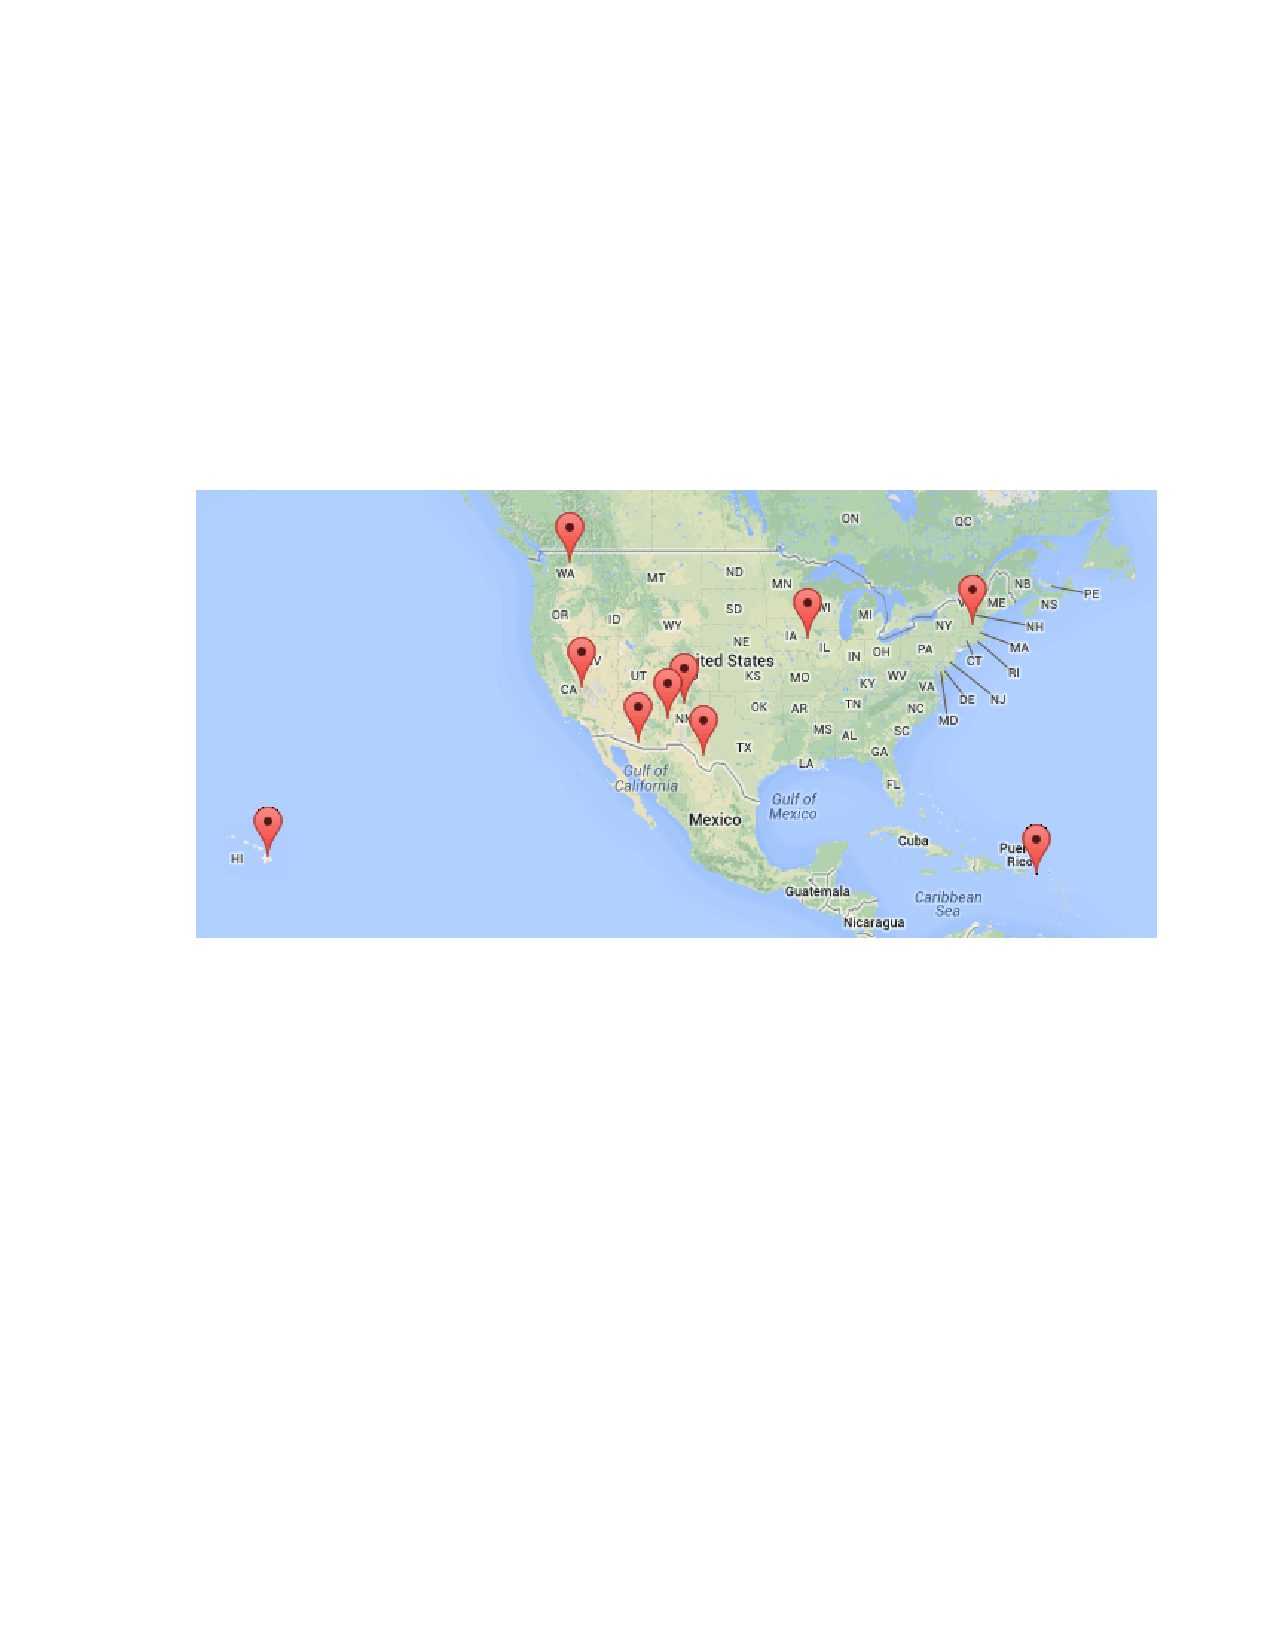
\includegraphics[width=\textwidth]{Images/C3/vlba.pdf}
  \caption{Telescope Locations in the Very Long Baseline Array}
  \label{fig: C3/vlba.pdf}
\end{figure}

The Very Long Baseline Interferometery or VLBI technique uses an array of antennas that are extremely far apart to achieve very high angular resolution images.
The Very Long Baseline Array, or VLBA, is a group of telescopes that are used at the same time to do VLBI.
Figure \ref{fig: C3/vlba.pdf} shows the locations of the VLBA telescopes.

